% !TeX spellcheck = es_ES
% !TEX encoding = UTF-8 Unicode
\documentclass[t, compress, spanish, aspectratio=169]{beamer}
%\documentclass[handout]{beamer}    % for the handout

\usetheme[progressbar=frametitle]{metropolis}

%\usetheme[secheader]{Madrid}
%\usetheme{Frankfurt}
%\usetheme{Warsaw}
%\usetheme{Berlin}
%\usetheme{CambridgeUS}

%\usecolortheme{beaver}     % Fondo Blanco y letras Negras - Titulos en Rojo con fondo gris
%\usecolortheme{dove}       % Para el Handout
%\usecolortheme{seahorse}   % Fondo Blanco y letras Negras - Titulos en Celeste
%\usecolortheme{dolphin}    % Fondo Blanco y letras Negras - Titulos en Celeste
%\usecolortheme{seagull}    % Fondo Blanco y letras Negras - Titulos en Gris
%\usecolortheme{crane}      % Fondo Blanco y letras Negras - Titulos en Amarillo
%\usecolortheme{wolverine}  % Fondo Blanco y Letras negras - Titulos en negro con fondo amarillo
%\usecolortheme{lily}       % Fondo Blanco y letras Negras - Titulos en Azul
%\usecolortheme{fly}        % Fondo Gris y letras Negras - Titulos en Rojo
%\usecolortheme{beetle}     % Fondo Gris y letras Negras - Titulos en blanco
%\usecolortheme{albatross}  % Fondo Azul y letras blancas
%\usecolortheme{orchid}     % Default
%\usecolortheme{rose}       % Default
%\usecolortheme{whale}      % Default

\setbeamertemplate{navigation symbols}{} % Gets rid of navigation symbols
%\setbeamercovered{transparent}

\usepackage{dsfont} % Double stroke fonts for math symbols
% \usepackage[T1]{fontenc}  % Helps with hyphenation for languages with accented characters. Note: Does not work with XeLaTex
% \usepackage[latin1]{inputenc} % Allows to type in latin (accents). Note: Does not work with XeLaTex
% \usefonttheme[onlymath]{serif}  % Changes fonts for math to serif
\usepackage[english]{babel} % Manages differences between languages: hyphenation etc

\usepackage{appendixnumberbeamer} % Does not include backup slides in the number of pages

\usepackage{centernot} % To draw not in math symbols (does not imply)

\usepackage{ragged2e}  % Text alignment
\justifying

\usepackage{graphicx} % Format for graphics: additional options for includefigure
\usepackage{pgf} % Tool for graphics

\usepackage{booktabs} % Format for tables: top, bottom and mid lines
\usepackage[scale=2]{ccicons}
\usepackage{threeparttable} % Format for tables
\usepackage{lscape} % Landscape for tables

% Customized commands
  \newcommand{\vs}{\vskip0pt plus.5fill}
  \newcommand{\SR}{\mathbb{R}}
  \DeclareMathOperator{\plim}{plim}
  \DeclareMathOperator{\Var}{Var}
  \DeclareMathOperator{\Avar}{AVar}
  \DeclareMathOperator{\Cov}{Cov}
  \DeclareMathOperator{\N}{Normal}
  \DeclareMathOperator{\E}{\mathbb{E}}
  \DeclareMathOperator{\LP}{\mathbb{L}}
  \newcommand{\pto}{\stackrel{p}{\longrightarrow}}
  \newcommand{\dto}{\stackrel{d}{\longrightarrow}}
  \newcommand{\adistr}{\stackrel{a}{\sim}}
  \newcommand{\epsi}{\varepsilon}
  \newcommand{\tmle}{\hat \theta_{ML}}
  \newcommand{\tgmm}{\hat \theta_{GMM}}
  \newcommand\independent{\protect\mathpalette{\protect\independenT}{\perp}}
  \def\independenT#1#2{\mathrel{\rlap{$#1#2$}\mkern2mu{#1#2}}}


\title [Temas adicionales MCO] {An\'alisis Econom\'etrico\\
Temas Adicionales MCO}
\author[de Elejalde]{Ramiro de Elejalde}
\institute [UAH] {Facultad de Econom\'ia y Finanzas \\ Universidad Alberto Hurtado}
\date[\today] {}
\subject{An\'alisis Econom\'etrico}
\begin{document}
	
%------------------------------------------------------------

\begin{frame}
    \titlepage
\end{frame}

% --------------------------------------------------- Slide --
\begin{frame}
	\frametitle{Outline}
	\tableofcontents
	\alert{Referencias}: Cap. 4.3.2 y 4.4 de Wooldridge, cap. 8 y 9 de Stock and Watson, y cap. 3.2.3 Angrist and Pischke.
\end{frame}
% --------------------------------------------------- Slide --
%\section{Variable proxy}
%\begin{frame}
%    \frametitle{Sesgo de variable omitida}
%    \begin{itemize}
%        \item Modelo de regresi\'on
%        \begin{align*}
%            y = \beta_0 + \beta_1 x_{1}+....+ \beta_K x_{K}+\gamma q +v,
%        \end{align*}
%        donde $\E(v|x)=0$.
%        \item No observamos $q$.
%        \item Soluci\'on 1: \alert{Estimamos el modelo por MCO sin $q$} $\implies$ \alert{Sesgo de variable omitida} (si $\Cov(q,x_j)\neq 0$ para alg\'un $j$).
%        \item Soluci\'on 2: \alert{Variable proxy $z$}.
%        
%        Supuestos
%        \begin{itemize}
%            \item Redundante: $\E(y|x,q,z)=\E(y|x,q)$,
%            \item Ausencia de correlaci\'on entre $x_j$ y $q$ una vez que controlamos por $z$:
%            \begin{align*}
%                q=\delta_0+\delta_1z+r,
%            \end{align*}
%            donde $\Cov(r,x_{j})=0$ para todo $j$.
%        \end{itemize}
%        La \alert{estimaci\'on es consistente}.
%    \end{itemize}
%\end{frame}
%% --------------------------------------------------- Slide --
%\begin{frame}
%    \frametitle{Sesgo de variable omitida}
%    \begin{itemize}
%        \item Soluci\'on 2: \alert{Variable proxy $z$}.
%        
%        Supuestos
%        \begin{itemize}
%        	\item Redundante: $\E(y|x,q,z)=\E(y|x,q)$,
%        	\item Ausencia de correlaci\'on entre $x_j$ y $q$ una vez que controlamos por $z$:
%        	\begin{align*}
%        	q=\delta_0+\delta_1z+r,
%        	\end{align*}
%        	donde $\Cov(r,x_{j})=0$ para todo $j$.
%        \end{itemize}
%        La \alert{estimaci\'on es consistente}.
%        \item Demostraci\'on
%        \begin{align*}
%            y = (\beta_0 +\gamma \delta_0)+ \beta_1 x_{1}+....+ \beta_K x_{K}+\gamma \delta_1 z+(\gamma r +v).
%        \end{align*}
%        Llamamos $u=\gamma r +v$. Tenemos 
%        \begin{align*}
%            \Cov(u,x_{j})&=\Cov(\gamma r +v,x_{j})=\gamma\Cov(r,x_{j})+\Cov(v,x_{j})=0,
%        \end{align*}
%        para  todo $j$.
%    \end{itemize}
%\end{frame}
%% --------------------------------------------------- Slide --
%\begin{frame}
%    \frametitle{Ejemplo: Efecto de capacitacion laboral en productividad}
%    \begin{itemize}
%        \item 157 firmas manufactureras de Michigan para los a\~nos 1987, 1988 y 1989.
%        \item 54 firmas reportaron la tasa de fallos en 1988.
%        \item En 1988, 19 de las 54 firmas tuvieron un subsidio para capacitaci\'on laboral.
%        \item Subsidio no fue asignado aleatoriamente.
%        \item Modelo
%        \begin{align*}
%            \log(scrap_i) = \beta_0 + \beta_1 grant_i+\gamma q_i +v_i,
%        \end{align*}
%        donde $scrap_i$ es el n\'umero de productos defectuosos cada 100 producidos y $grant_i$ es una dummy si le otorgaron el subsidio a la firma. 
%        \item Variable proxy: $\log(scrap_{-1,i})$.
%    \end{itemize}
%\end{frame}
%% --------------------------------------------------- Slide --
%\begin{frame}[fragile]
%\frametitle{Estimaci\'on MCO: Efecto de capacitacion laboral en productividad}
%\begin{itemize}
%\item [] Salida de Stata\\
%\tiny{
%\begin{verbatim}
%
%
%.         reg lscrap grant if year==1988, robust
%
%Linear regression                                      Number of obs =      54
%                                                       F(  1,    52) =    0.02
%                                                       Prob > F      =  0.8793
%                                                       R-squared     =  0.0004
%                                                       Root MSE      =  1.4232
%
%------------------------------------------------------------------------------
%             |               Robust
%      lscrap |      Coef.   Std. Err.      t    P>|t|     [95% Conf. Interval]
%-------------+----------------------------------------------------------------
%       grant |   .0566004   .3708355     0.15   0.879    -.6875354    .8007362
%       _cons |    .408526    .262929     1.55   0.126    -.1190797    .9361317
%------------------------------------------------------------------------------
%\end{verbatim}
%}
%\end{itemize}
%\end{frame}
%% --------------------------------------------------- Slide --
%\begin{frame}[fragile]
%\frametitle{Estimaci\'on MCO: Efecto de capacitacion laboral en productividad}
%\begin{itemize}
%\item [] Salida de Stata\\
%\tiny{
%
%\begin{verbatim}
%
%.         reg lscrap grant lscrap_1 if year==1988, robust
%
%Linear regression                                      Number of obs =      54
%                                                       F(  2,    51) =   77.79
%                                                       Prob > F      =  0.0000
%                                                       R-squared     =  0.8728
%                                                       Root MSE      =  .51267
%
%------------------------------------------------------------------------------
%             |               Robust
%      lscrap |      Coef.   Std. Err.      t    P>|t|     [95% Conf. Interval]
%-------------+----------------------------------------------------------------
%       grant |  -.2539697   .1463727    -1.74   0.089    -.5478251    .0398857
%    lscrap_1 |   .8311606   .0735407    11.30   0.000     .6835215    .9787996
%       _cons |    .021237   .0998451     0.21   0.832    -.1792103    .2216843
%------------------------------------------------------------------------------
%
%\end{verbatim}
%}
%\end{itemize}
%\end{frame}
% --------------------------------------------------- Slide --
\section{Error de medida}
\begin{frame}
    \frametitle{Error de medida en la variable dependiente}
    \small
    \begin{itemize}  
        \item Modelo de regresi\'on
        \begin{align*}
            y^* = \beta_0 + \beta_1 x_{1}+....+ \beta_K x_{K}+v,
        \end{align*}
        donde $\Cov(v, x_{j})=0$ para todo $j$.
        \item No observamos $y^*$ pero observamos un medida de $y^*$ dada por $y$.
        \item Definimos el error de medida poblacional como,
        \begin{align*}
            e_{0} = y-y^*.
        \end{align*}
        \item [] El modelo que podemos estimar es,
        \begin{align*}
            y = \beta_0 + \beta_1 x_{1}+....+ \beta_K x_{K}+v+e_{0}.
        \end{align*}
        \item ?`Es la estimaci\'on MCO consistente?
        \end{itemize}
\end{frame}

%\begin{frame}
%    \frametitle{Error de medida en la variable dependiente}
%\end{frame}
%
%\begin{frame}
%    \frametitle{Error de medida en la variable dependiente}
%\end{frame}
%
%
%\begin{frame}
%    \frametitle{Error de medida en la variable dependiente}
%\end{frame}

\begin{frame}
    \frametitle{Error de medida en la variable dependiente}
    \small
    \begin{itemize}  
        \item Modelo de regresi\'on
        \begin{align*}
            y^* = \beta_0 + \beta_1 x_{1}+....+ \beta_K x_{K}+v,
        \end{align*}
        donde $\Cov(v, x_{j})=0$ para todo $j$.
        \item No observamos $y^*$ pero observamos un medida de $y^*$ dada por $y$.
        \item Definimos el error de medida poblacional como,
        \begin{align*}
            e_{0} = y-y^*.
        \end{align*}
        \item [] El modelo que podemos estimar es,
        \begin{align*}
            y = \beta_0 + \beta_1 x_{1}+....+ \beta_K x_{K}+v+e_{0}.
        \end{align*}
        \item ?`Es la estimaci\'on MCO consistente? Si, si el error de medida no est\'a correlado con las $x$'s, $\Cov(x_{j},e_{0})=0$ para todo $j$.
        \item Mayor varianza del error: Si $\Cov(v, e_{0})=0$, $\Var(v+e_{0})=\Var(v)+\Var(e_{0})\geq \Var(v)$.    
        \end{itemize}
\end{frame}


% --------------------------------------------------- Slide --
\begin{frame}
    \frametitle{Error de medida en la variable explicativa}
    \small
    \begin{itemize} 
        \item Modelo de regresi\'on
        \begin{align*}
            y = \beta_0 + \beta_1 x_{1}^*+....+ \beta_K x_{K}+v,
        \end{align*}
        donde $\Cov(v, x_j)=0$ para todo $j\neq 1$ y $\Cov(v, x_{1}^*)=0$.
        \item No observamos $x_{1}^*$ pero observamos un medida de $x_{1}^*$ dada por $x_{1}$. 
        Suponemos que $\Cov(x_{1},v)=0$.
        \item Definimos el error de medida poblacional como,
        \begin{align*}
            e_{1} = x_{1}-x^*_{1},
        \end{align*}
        donde $\E(e_{1})=0$. Dados los supuestos anteriores, $\Cov(e_{1}, v)=0$.
        % Si no se verifica afecta a la constante.
        \item [] El modelo que podemos estimar es,
        \begin{align*}
            y = \beta_0 + \beta_1 x_{1}+....+ \beta_K x_{K}+(v-\beta_1 e_{1}).
        \end{align*}
        \item ?`Es la estimaci\'on MCO consistente?
\end{itemize}
\end{frame}
% --------------------------------------------------- Slide --
\begin{frame}
	\frametitle{Error de medida en la variable explicativa}
	?`Es la estimaci\'on MCO consistente? Suponemos que $\Cov(x_{j},e_{1})=0$ para todo $j\neq 1$. El supuesto clave es la relaci\'on entre $e_{1}$ con $x_{1}$ y $x^*_{1}$
	\begin{itemize}  
			\item \alert{Error de medida no est\'a correlado con la variable observada}: $\Cov(x_{1},e_{1})=0$.
			\item [] Es consistente pero hay una pérdida de eficiencia.
			\item \alert{Error de medida cl\'asico}: Error de medida no est\'a correlado con la variable NO observada, $\Cov(x_{1}^*,e_{1})=0$.
			\item [] No es consistente $\implies$ \alert{Sesgo de atenuación}
	\end{itemize}
\end{frame}

%\begin{frame}
%	\frametitle{Error de medida no est\'a correlado con la variable observada: $\Cov(x_{1},e_{1})=0$}
%\end{frame}
%
%\begin{frame}
%	\frametitle{Error de medida no est\'a correlado con la variable observada: $\Cov(x_{1},e_{1})=0$}
%\end{frame}
%
%\begin{frame}
%	\frametitle{Error de medida no est\'a correlado con la variable observada: $\Cov(x_{1},e_{1})=0$}
%\end{frame}


% --------------------------------------------------- Slide --
\begin{frame}
    \frametitle{Error de medida no est\'a correlado con la variable observada: $\Cov(x_{1},e_{1})=0$}
    \begin{itemize}  
    	\item[]
            \begin{align*}
                \Cov(x_{1}, u) &=\Cov(x_{1}, (v-\beta_1 e_{1})),\\
                               &=\Cov(x_{1},v)-\beta_1 \Cov(x_{1},e_{1}),\\
                               &=0.
            \end{align*}
            \item MCO es \alert{consistente pero la varianza del error es mayor} $\Var(v-\beta_1 e_{1})=\Var(v)+\beta_1^2 \Var(e_{1})$.
\end{itemize}
\end{frame}
% --------------------------------------------------- Slide --
%\begin{frame}
%    \frametitle{Error de medida cl\'asico: $\Cov(x_{1}^*,e_{1})=0$}
%\end{frame}
%
%\begin{frame}
%    \frametitle{Error de medida cl\'asico: $\Cov(x_{1}^*,e_{1})=0$}
%\end{frame}
%
%\begin{frame}
%    \frametitle{Error de medida cl\'asico: $\Cov(x_{1}^*,e_{1})=0$}
%\end{frame}
%
%\begin{frame}
%    \frametitle{Error de medida cl\'asico: $\Cov(x_{1}^*,e_{1})=0$}
%\end{frame}

\begin{frame}
    \frametitle{Error de medida cl\'asico: $\Cov(x_{1}^*,e_{1})=0$}
    \begin{itemize}  
            \item []
            \begin{align*}
                \Cov(x_{1}, e_{1}) &=\Cov((x_{1}^*+e_{1}), e_{1}),\\
                               &=\Cov(x_{1}^*,e_{1})+\Var(e_{1}),\\
                               &=\Var(e_{1}).
            \end{align*}
            \item Entonces $\Cov(x_{1}, (v-\beta_1 e_{1}))=-\beta_1 \Var(e_{1})$ y MCO es \alert{inconsistente} para todos los $\beta$'s.
            \item Sesgo asint\'otico? $\implies$ \alert{Sesgo de atenuaci\'on}.
\end{itemize}
\end{frame}

% --------------------------------------------------- Slide --
\begin{frame}
	\frametitle{Error de medida cl\'asico: $\Cov(x_{1}^*,e_{1})=0$}
	\begin{itemize}  
		\item Sesgo asint\'otico? $\implies$ \alert{Sesgo de atenuaci\'on}.
		\small
		\item [] Demostraci\'on (sketch para el modelo de regresi\'on simple $y=\beta_0+\beta_1 x_1^*+v$):
		\begin{align*}
		\plim \hat \beta_1 &= \frac{\Cov(x_1, y)}{\Var(x_1)},\\
		&= \frac{\Cov( x_1,\beta_0 + \beta_1 x_{1}+(v-\beta_1 e_{1}) )}{\Var( x_1)},\\
		&= \beta_1+\frac{\Cov(x_1,(v-\beta_1 e_{1}) )}{\Var(x_1)},\\
		&= \beta_1-\beta_1 \frac{\Var(e_{1})}{\Var(x_1)},\\
		&=\beta_1\left(1-\frac{\Var(e_{1})}{\Var(x_1)} \right),\\
		&=\beta_1\left(\frac{\Var(x_1^*)}{\Var(x_1^*)+\Var(e_{1})} \right).\\
		\end{align*}
	\end{itemize}
\end{frame}

% --------------------------------------------------- Slide --
\section{M\'inimos cuadrados generalizados (GLS)}
\begin{frame}
    \frametitle{M\'inimos cuadrados generalizados (GLS)}
    \begin{itemize}
    \item []
    \begin{align*}
        y_i=\beta_0 + \beta_1 x_{1i} + ...+\beta_K  x_{Ki}+u_i = x_i'\beta+u_i,
    \end{align*}
    donde $y_i$ es una variable aleatoria, $x_i$ es un vector aleatorio de $K \times 1$ y $u_i$ es una variable aleatoria.
    \item <2->\alert{Supuestos}:
    \begin{enumerate}
        \bigskip
        \item [GLS1] Muestra aleatoria de tama\~no $N$ $\implies \{y_i,x_i\}_{i=1}^N$ i.i.d.,
        \bigskip
        \item [GLS2] Independencia en media: $\E(u_i|x_i)=0$,
        \bigskip
        \item [GLS3] $\Var(u_i|x_i)=\sigma^2(x_i)$,
        \bigskip
        \item [GLS4] $\E \left(\frac{x_ix_i'}{\sigma^2(x_i)}\right)$ no singular.
        \bigskip
    \end{enumerate}
    \end{itemize}
\end{frame}
% --------------------------------------------------- Slide --
\begin{frame}
    \frametitle{M\'inimos cuadrados generalizados (GLS)}
    \begin{itemize}
    \item Idea: Transformar el modelo en homosced\'astico y luego aplicar MCO que sabemos es eficiente bajo homoscedasticidad e independencia en media.
    \end{itemize}
\end{frame}

%\begin{frame}
%    \frametitle{M\'inimos cuadrados generalizados (GLS)}
%\end{frame}

\begin{frame}
    \frametitle{M\'inimos cuadrados generalizados (GLS)}
    \begin{itemize}
    \item Idea: Transformar el modelo en homosced\'astico y luego aplicar MCO que sabemos es eficiente bajo homoscedasticidad e independencia en media.
    \item []
        \begin{align*}
            \frac{y_i}{\sigma(x_i)}= \frac{x_i}{\sigma(x_i)}'\beta+\frac{u_i}{\sigma(x_i)},
        \end{align*}
        donde 
        \begin{align*}
            \Var\left(\frac{u_i}{\sigma(x_i)}|x_i\right)&=\E\left(\frac{u_i^2}{\sigma^2(x_i)}|x_i\right),\\
                                                    &=\frac{\E(u_i^2|x_i)}{\sigma^2(x_i)},\\
                                                    &=1.
        \end{align*}
    \end{itemize}
\end{frame}

\begin{frame}
    \frametitle{M\'inimos cuadrados generalizados (GLS)}
    \begin{itemize}
    \item  Estimador por GLS
    \begin{align*}
        \hat \beta_{GLS} =\left(\frac{1}{N}\sum_{i=1}^{N} \frac{x_ix_i'}{\sigma^2(x_i)}\right)^{-1} \frac{1}{N} \sum_{i=1}^{N} \frac{x_iy_i}{\sigma^2(x_i)}.
    \end{align*}
    \end{itemize}
\end{frame}
% --------------------------------------------------- Slide --
%\begin{frame}
%    \frametitle{Propiedades: Consistencia}
%\end{frame}

\begin{frame}
    \frametitle{Propiedades: Consistencia}
        \begin{align*}
            \plim \hat \beta_{GLS} & = \plim\left[ \left( \frac{1}{N}\sum_{i=1}^{N} \frac{x_ix_i'}{\sigma^2(x_i)}\right)^{-1}\left( \frac{1}{N} \sum_{i=1}^{N} \frac{x_iy_i}{\sigma^2(x_i)}\right)\right],\\
            & = \beta + \left( \plim \frac{1}{N}\sum_{i=1}^{N} \frac{x_ix_i'}{\sigma^2(x_i)}\right)^{-1}\plim\left( \frac{1}{N} \sum_{i=1}^{N} \frac{x_iu_i}{\sigma^2(x_i)}\right),\\
            & = \beta,
        \end{align*}
        usando LGN, TFC y $\E(u_i|x_i)=0$.
\end{frame}
%Necesitamos imponer un supuesto mas fuerte de independencia en media.
% --------------------------------------------------- Slide --
%\begin{frame}
%    \frametitle{Propiedades: Distribuci\'on asint\'otica normal} 
%\end{frame}
%
%\begin{frame}
%    \frametitle{Propiedades: Distribuci\'on asint\'otica normal} 
%\end{frame}

\begin{frame}
    \frametitle{Propiedades: Distribuci\'on asint\'otica normal} 
    \small
        \begin{align*}
            \sqrt{N} (\hat \beta_{GLS} - \beta)&= \left( \frac{1}{N}\sum_{i=1}^{N} \frac{x_ix_i'}{\sigma^2(x_i)}\right)^{-1 }N^{1/2} \frac{1}{N} \sum_{i=1}^{N} \frac{x_iu_i}{\sigma^2(x_i)}.
        \end{align*}
        Usando LGN y TCL tenemos,
        \begin{align*}
            N^{1/2} \frac{1}{N} \sum_{i=1}^{N} \frac{x_iu_i}{\sigma^2(x_i)} &\dto \N \left(0,\E\left(\frac{u_i^2}{\sigma^2(x_i)} \frac{x_i x_i'}{\sigma^2(x_i)}\right)\right),\\
            &\dto \N \left(0,\E\left(\frac{x_i x_i'}{\sigma^2(x_i)}\right)\right),\\
           \left( \frac{1}{N}\sum_{i=1}^{N} \frac{x_ix_i'}{\sigma^2(x_i)}\right)^{-1 }&\pto  \E\left(\frac{x_ix_i'}{\sigma^2(x_i)}\right)^{-1 } .
        \end{align*}
        Usando el teorema de Slutsky
        \begin{align*}
            \sqrt{N} (\hat \beta_{GLS} - \beta) &\dto \N \left(0,\E\left(\frac{x_i x_i'}{\sigma^2(x_i)}\right)^{-1}\right).
        \end{align*}
\end{frame}
% --------------------------------------------------- Slide --
\begin{frame}
    \frametitle{M\'inimos cuadrados generalizados factibles (FGLS)}
    \begin{itemize}
        \item  En la pr\'actica no conocemos $\sigma^2(x_i)$.
        \item []Si suponemos una forma funcional $\sigma^2(x_i, \gamma)$, podemos estimar $\sigma^2(x_i, \gamma)$ consistentemente usando los residuos de la estimaci\'on por MCO,
        \begin{align*}
            \hat u_i^2=\sigma^2(x_i, \gamma)+error.
        \end{align*}
        \item []Luego podemos estimar por $GLS$ usando $\sigma^2(x_i, \hat \gamma)$: \alert{M\'inimos cuadrados generalizados factibles}.
        \item  []Se puede demostrar que $GLS$ y $FGLS$ son asint\'oticamente equivalentes.
        \item []En la pr\'actica es preferible utilizar errores robustos.
    \end{itemize}
\end{frame}
%% --------------------------------------------------- Slide --
%\subsection{Test de Heteroscedasticidad}
%
%\begin{frame} [fragile]
%    \frametitle{Test de Heteroscedasticidad}
%    \begin{itemize}
%        \item <1-> Dado el modelo,
%        \begin{align*}
%            y_i=\beta'x_i+u_i,
%        \end{align*}
%        donde $\E(u_i|x_i)=0$.
%        \item <2-> Contraste de  hip\'otesis: $H_0:\E(u_i^2|x_i)=\sigma^2$.
%        \item <3-> []Dado una funci\'on de $x_i$, $h(x_i)$ bajo la hip\'otesis nula $\Cov(u_i^2,h(x_i))=0$.
%        \item <4-> []Podemos utilizar el modelo:
%        \begin{align*}
%            u_i^2=\delta_0+h(x_i)'\delta+v_i,
%        \end{align*}
%        bajo los supuestos usuales.
%        \item <5-> []Bajo $H_0$, tenemos que $\delta_0=\sigma^2$ y $\delta=0$, y podemos hacer un test multiplicadores de Lagrange ($LM_N$) del tipo $H_0:\delta=0$.
%        \item <6-> En realidad no observamos $u_i^2$ pero lo podemos reemplazar por $\hat u_i^2$ y asint\'oticamente nada cambia.
%        \item <7-> Cuando $h(x_i)=x_i$ tenemos el test de Breusch-Pagan, y para $h(x_i)$ incluye $x_i$ y $x_ix_i'$ tenemos el test de White.
%        \item <8-> En Stata despues de reg usamos \verb|estat hettest, iid|.
%    \end{itemize}
%\end{frame}
%% --------------------------------------------------- Slide --
%\begin{frame}
%    \frametitle{Propiedades}
%    \begin{itemize}
%        \item <1-> Distribuci\'on asint\'otica normal
%        \begin{align*}
%            \sqrt{N} (\hat \beta_{GLS} - \beta)&= \left( \frac{1}{N}\sum_{i=1}^{N} \frac{x_ix_i'}{\sigma^2(x_i)}\right)^{-1 }N^{1/2} \frac{1}{N} \sum_{i=1}^{N} \frac{x_iu_i}{\sigma^2(x_i)}.
%        \end{align*}
%        Usando LGN y TCL en,
%        \begin{align*}
%            N^{1/2} \frac{1}{N} \sum_{i=1}^{N} \frac{x_iu_i}{\sigma^2(x_i)} &\dto \N \left(0,\E\left[\frac{u_i^2}{\sigma^2(x_i)} \frac{x_i x_i'}{\sigma^2(x_i)}\right]\right),\\
%            &\dto \N \left(0,\E\left[\frac{x_i x_i'}{\sigma^2(x_i)}\right]\right).
%        \end{align*}
%        Usando el teorema de Slutsky
%        \begin{align*}
%            \sqrt{N} (\hat \beta_{GLS} - \beta) &\dto \N \left(0,\E\left[\frac{x_i x_i'}{\sigma^2(x_i)}\right]^{-1}\right).
%        \end{align*}
%    \end{itemize}
%\end{frame}
%% --------------------------------------------------- Slide --
%\begin{frame}
%    \frametitle{M\'inimos cuadrados generalizados factibles (FGLS)}
%    \begin{itemize}
%        \item <1-> En la pr\'actica no conocemos $\sigma^2(x_i)$.
%        \item <2-> []Si suponemos una forma funcional $\sigma^2(x_i, \gamma)$, podemos estimar $\sigma^2(x_i, \gamma)$ consistentemente usando los residuos de la estimaci\'on por MCO,
%        \begin{align*}
%            \hat u_i^2=\sigma^2(x_i, \gamma)+error.
%        \end{align*}
%        \item <3-> []Luego podemos estimar por $GLS$ usando $\sigma^2(x_i, \hat \gamma)$: M\'inimos cuadrados factibles.
%        \item <4-> []Se puede demostrar que $GLS$ y $FGLS$ son asint\'oticamente equivalentes.
%        \item <5-> []En la pr\'actica es preferible utilizar errores robustos.
%    \end{itemize}
%\end{frame}
% --------------------------------------------------- Slide --
\begin{frame}
    \frametitle{Test de Heteroscedasticidad}
    \begin{itemize}
        \small
        \item  Dado el modelo,
        \begin{align*}
            y_i=\beta'x_i+u_i,
        \end{align*}
        donde $\E(u_i|x_i)=0$.
        \item  \alert{Contraste de  hip\'otesis}: $H_0:\E(u_i^2|x_i)=\sigma^2$.
        \item  []Dado una funci\'on de $x_i$, $h(x_i)$ bajo la hip\'otesis nula $\Cov(u_i^2,h(x_i))=0$.
        \item  []Podemos utilizar el modelo:
        \begin{align*}
            u_i^2=\delta_0+h(x_i)'\delta+v_i,
        \end{align*}
        bajo los supuestos usuales.
        \item  []Bajo $H_0$, tenemos que $\delta_0=\sigma^2$ y $\delta=0$, y podemos hacer el contraste $H_0:\delta=0$ utilizando un test multiplicadores de Lagrange ($LM_N=N \hat R^2 \pto \chi^2_q$).
        \item  En realidad no observamos $u_i^2$ pero lo podemos reemplazar por $\hat u_i^2$ y asint\'oticamente nada cambia.
    \end{itemize}
\end{frame}
% --------------------------------------------------- Slide --
\begin{frame}[fragile]
    \frametitle{Test de Heteroscedasticidad}
    \begin{itemize}
        \item  Dado el modelo,
        \begin{align*}
            y_i=\beta'x_i+u_i,
        \end{align*}
        donde $\E(u_i|x_i)=0$.
        \item  Contraste de  hip\'otesis: $H_0:\E(u_i^2|x_i)=\sigma^2$.
        \item Cuando $h(x_i)=x_i$ tenemos el test de Breusch-Pagan, y para $h(x_i)$ incluye $x_i$ y $x_ix_i'$ tenemos el test de White.
        \item  En Stata despues de reg usamos \verb|estat hettest, iid|.
    \end{itemize}
\end{frame}
% --------------------------------------------------- Slide --
\section{Validaci\'on interna y validaci\'on externa}
\begin{frame}
    \frametitle{Validaci\'on interna y validaci\'on externa}
    \begin{itemize}
        \item \alert{Validez interna}: la inferencia estad\'istica de los efectos causales de inter\'es son v\'alidos para la poblaci\'on estudiada.
        \item \alert{Validez externa}: la inferencia estad\'istica sobre los efectos causales se puede generalizar a poblaciones con diferentes condiciones institucionales, legales, sociales y econ\'omicas.
    \end{itemize}
\end{frame}
% --------------------------------------------------- Slide --
\begin{frame}
    \frametitle{Amenazas a la validaci\'on externa}
    \begin{itemize}
        \item  Diferencias entre la poblaci\'on y contexto estudiados, y la poblaci\'on y contexto de inter\'es.
        \begin{itemize}
            \item Diferencias en las poblaciones: Efectos sobre alumnos en escuela media.
            \item Diferencias en las condiciones institucionales, legales, sociales y econ\'omicas: diferentes caracter\'isticas de los profesores, escuelas privadas y p\'ublicas, etc.
        \end{itemize}
        \item ?`C\'omo evaluar la validez externa?
        \begin{itemize}
            \item Evaluar si hay diferencias importantes entre la poblaci\'on bajo estudio y la poblaci\'on de inter\'es.
            \item Comparar resultados de estudios similares en poblaciones diferentes.
            % Efecto del tama\~no de clase en Massachusetts
        \end{itemize}
    \end{itemize}
\end{frame}
% --------------------------------------------------- Slide --
\begin{frame}
    \frametitle{Amenazas a la validaci\'on interna}
    \begin{itemize}
        \item Sesgo por omisi\'on de variable
        \item Mala especificaci\'on de la forma funcional
        \item Sesgo por error de medida
        \item Sesgo por selecci\'on de muestra
        \item Sesgo por simultaneidad
        \item [] Nota: Todas estos problemas generan correlaci\'on entre variables explicativas y el error, y se suelen llamar \alert{problemas de endogeneidad}.
    \end{itemize}
\end{frame}
% 1. El estimador debe ser consistente
% 2. Los test deben tener el nivel de significatividad deseado. (La estimaci\'on de los s.e. debe ser consistente.) Por ejemplo, asumimos homoscedasticidad cuando el modelo es heteroscedastico.
% --------------------------------------------------- Slide --
\begin{frame}
    \frametitle{Sesgo por omisi\'on de variable}
    \begin{itemize}
        \item Surge si una variable omitida
        \begin{itemize}
            \item Est\'a correlada con la variable dependiente $y$
            \item Est\'a correlada con al menos una variable explicativa $x_{j}$.
        \end{itemize}
        \item Soluciones
        \begin{itemize}
            \item Si la variable puede ser medida, incluirla en la regresi\'on como variable explicativa adicional.
            % Trade-off sesgo vesus efeciencia (omisi\'on de variable relevante vs incluir variable irrelevante)
            % 1. Identificar los coeficientes de interes
            % 2. Determinar a priori, los factores omitidos que puede generar un sesgo por omisi\'on de variable.
            % 3. Contrastar si las variables inclu\'idas son significativas o el coeficiente de interes cambia
            % 4. Mostrar los resultados de varias especificaciones para que el lector pueda evaluar la robustez de los resultados.
            \item Si tenemos una buena proxy, utilizar la proxy en la regresi\'on como variable explicativa adicional.
            \item Utilizar \alert{variables intrumentales} (el tema de la siguiente unidad del curso).
            \item Si observamos la misma unidad en distintos momentos del tiempo utilizar \alert{datos de panel} que nos permite controlar por factores inobservados que permanecen fijos a lo largo del tiempo (el tema de Econometr\'ia II).
            \item Realizar un experimento aleatorio controlado (\alert{randomized controlled experiment}).
        \end{itemize}
    \end{itemize}
\end{frame}
% --------------------------------------------------- Slide --
\begin{frame}
    \frametitle{Mala especificaci\'on de la forma funcional}
    \begin{itemize}
        \item Surge si la forma funcional de la esperanza condicional no es lineal.
        % Aunque siempre podemos justificar que el modelo de regresi\'on es la mejor aproximaci\'on lineal al modelo de esperanza condicional.
        \item Soluciones
        \begin{itemize}
            \item Variable dependiente continua: utilizar una forma no lineal apropiada: logaritmos, polinomios, interacciones,etc.
            % Para detectar la formas funcional adecuada:
            % 1. Graficar los datos (y versus x_j,\'o u versus x_j)
            % 2. En caso de modelos anidados, contrastar sin los polinomios adicionales son significativos o test mas generales como RESET.
            % 3. En caso de modelos no anidados, existen test para este tipo de contraste como Box-Cox
            \item Variable dependiente discreta: modelos econom\'etricos espec\'ificos para este tipo de variables. Por ejemplo, para variables binarias tenemos el modelo Logit y Probit (el tema de la \'ultima unidad del curso).
        \end{itemize}
    \end{itemize}
\end{frame}
% --------------------------------------------------- Slide --
\begin{frame}
    \frametitle{Sesgo por error de medida}
    \begin{itemize}
        \item Surge por error de medida en las variables por problemas en el registro de datos administrativos, en la recolecci\'on de datos de las encuestas, en el ``wording'' de las preguntas, respuestas intencionalmente falsas, etc.
        % Ejmplo: Ingresos: si es declarado por la persona puede tener error porque las personas no recuerdan con exactitud cuanto ganaron, porque reporten el ingreso en forma err\'onea, si son datos administrativos puede ser por error en la entrada de datos.
        \item Soluciones
        \begin{itemize}
            \item Obtener mejores datos.
            \item Utilizar \alert{variables instrumentales}.
        \end{itemize}
    \end{itemize}
\end{frame}
% --------------------------------------------------- Slide --
\begin{frame}
    \frametitle{Sesgo por selecci\'on de muestra}
    \begin{itemize}
        \item El sesgo por selecci\'on de muestra surge si la disponibilidad datos depende de un proceso de selecci\'on que est\'a relacionado con la variable dependiente.
        % Genera correlaci\'on entre el error y la variable explicativa.
        % Por ejemplo, efecto de salarios en educaci\'on.
        % Factores observados e inobservados que afectan la posibilidad que una persona est\'e empleada a su vez afectan el salario que puede recibir la persona.
        \item Soluciones
        \begin{itemize}
            \item Recolectar los datos de forma tal de aliviar el problema de selecci\'on
            \item Construir un modelo del proceso de selecci\'on y estimarlo (Heckman).
            \item Realizar un experimento aleatorio controlado.
        \end{itemize}
    \end{itemize}
\end{frame}
% --------------------------------------------------- Slide --
\begin{frame}
    \frametitle{Sesgo por simultaneidad}
    \begin{itemize}
        \item Hasta ahora hemos supuesto que $x$ causa a $y$ .?`Qu\'e pasa si $y$ causa a $x$? \alert{(feedback effect)}
        % Ejemplo: Subsidio del gobierno para contratar profesores en escuelas con malos resultados acad\'emicos.
        \item Soluciones
        \begin{itemize}
            \item Realizar un experimento aleatorio controlado.
            \item Estimar un modelo completo con las ambas causalidades: Sistema de ecuaciones.
            \item Utilizar variables instrumentales.
        \end{itemize}
    \end{itemize}
\end{frame}
% --------------------------------------------------- Slide --
\begin{frame}
    \frametitle{Inconsistencia en la estimaci\'on de los errores est\'andar}
    \begin{itemize}
        \item Heterocedasticidad
        \item Correlaci\'on del t\'ermino de error entre observaciones: Datos de panel y series de tiempo.
        % Errores robustos a la correlaci\'on serial para datos de panel y HAC para series temporales. 
    \end{itemize}
\end{frame}
% --------------------------------------------------- Slide --
\begin{frame}
    \frametitle{Ejemplo: Tama\~no de clase y rendimiento acad\'emico para California}
    \begin{itemize}
        \item \alert{Objetivo}: Analizar las amenazas a la validez interna y externa en los resultados emp\'iricos con los datos de California.
        \item \alert{Validez externa}
        \begin{itemize}
            \item Comparar los resultados de California con los resultados de Massachusetts.
        \end{itemize}
        % Depende del contexto en que queremos hacer la generalizacion, en este caso nos referimos a otros distritos de escuelas publicas primarias de USA
        \item \alert{Validez interna}
        \begin{itemize}
            \item Evaluar la lista de 5 amenazas a la validez interna.
        \end{itemize}
    \end{itemize}
\end{frame}
% --------------------------------------------------- Slide --
\begin{frame}
    \frametitle{Forma funcional}
    \begin{itemize}
        \item ?`Efecto del ingreso en el rendimiento acad\'emico es lineal?
        \item ?`Efecto marginal de aumentar el tama\~no del clase depende del porcentaje de ni\~nos que deben aprenden ingl\'es?
        \item ?`Efecto marginal de aumentar el tama\~no del clase depende del tama\~no de clase?
    \end{itemize}
\end{frame}
% --------------------------------------------------- Slide --
\begin{frame}
    \frametitle{Forma funcional}
    \begin{itemize}
        \item Teor\'ia econ\'omica puede sugerir la forma funcional.
        \item An\'alisis gr\'afico puede ayudar en determinar la forma funcional.
        % Explicativas contra dependientes
        % Explicativa filtrada contra dependiente filtrada: partial regression plots (avplot avginc)
        \item Si la variable dependientes es la misma y los modelos alternativos son anidados, podemos utilizar un test de Wald.
        \item Si la variable dependientes es la misma pero los modelos no son anidados, podemos utilizar el $R^2$ ajustado.
        \item Si la variable dependiente es distinta, podemos utilizar un test del modelo de Box-Cox
        % ()y^\theta-1)/\theta: \theta=1 es lineal, \theta=0 es log. Es un modelo no lineal pero se puede estimar con el comando boxcox.
    \end{itemize}
\end{frame}
% --------------------------------------------------- Slide --
\begin{frame}
    \frametitle{Efecto del ingreso}
    \vspace{-0.5cm}
    \begin{figure}[h!]
          \caption{Scatter plot: Lineal, nivel-log, cuadr\'atico}
          \centering
          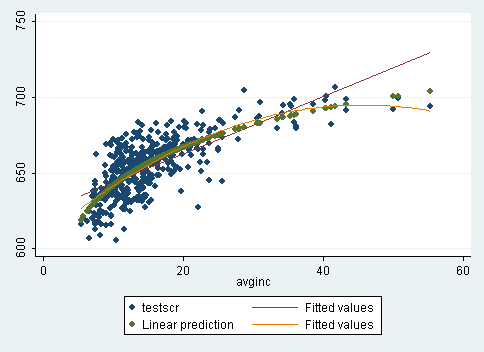
\includegraphics[width=0.70\textwidth]{figures/test_income.png}
    \end{figure}
\end{frame}
% --------------------------------------------------- Slide --
\begin{frame}
    \frametitle{Efecto del ingreso}
    \vspace{-0.5cm}
    \begin{figure}[h!]
          \caption{Regresi\'on particionada: avplot avginc }
          \centering
          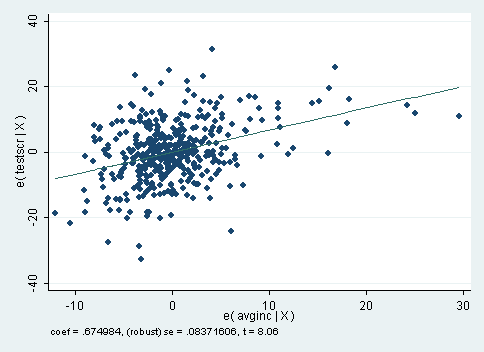
\includegraphics[width=0.70\textwidth]{figures/partial_regression_plot_income.png}
    \end{figure}
\end{frame}

% --------------------------------------------------- Slide --
\begin{frame}
    \frametitle{Efecto del ingreso}
    \vspace{-0.5cm}
    \begin{figure}[h!]
          \caption{Valores predichos y residuos: rvfplot}
          \centering
          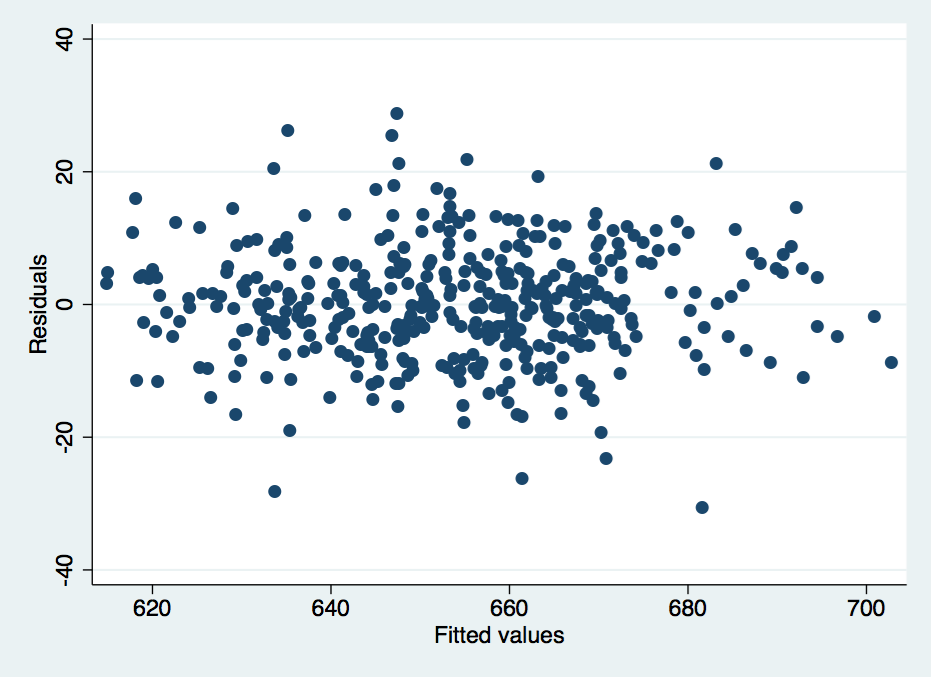
\includegraphics[width=0.70\textwidth]{figures/fitted_residuals_plot_income.png}
    \end{figure}
\end{frame}


% --------------------------------------------------- Slide --
\begin{frame}  [fragile]
    \frametitle{Estimaci\'on MCO}
    \tiny{
    \begin{verbatim}
------------------------------------------------------------------------------------
                          Model 1         Model 2         Model 3         Model 4   
------------------------------------------------------------------------------------
Stud/teacher (str)         -0.998***       -0.734***       -0.947***       65.286** 
                          (0.270)         (0.257)         (0.347)        (25.259)   
English learn % (el)       -0.122***       -0.176***       -0.482*         -0.166***
                          (0.033)         (0.034)         (0.246)         (0.034)   
Lunch subsidy              -0.547***       -0.398***       -0.401***       -0.402***
                          (0.024)         (0.033)         (0.033)         (0.033)   
Log(Average income)                        11.569***       11.433***       11.509***
                                          (1.819)         (1.818)         (1.806)   
el X str                                                    0.015                   
                                                          (0.012)                   
str^2                                                                      -3.466***
                                                                          (1.271)   
str^3                                                                       0.060***
                                                                          (0.021)   
Constant                  700.150***      658.552***      663.158***      244.803   
                          (5.568)         (8.642)        (10.054)       (165.722)   
------------------------------------------------------------------------------------
R-squared                   0.775           0.796           0.797           0.801   
N                         420.000         420.000         420.000         420.000   
------------------------------------------------------------------------------------
* p<0.10, ** p<0.05, *** p<0.01
    \end{verbatim}
    }
\end{frame}
% --------------------------------------------------- Slide --
\begin{frame}  [fragile]
    \frametitle{Efectos marginales de Student/teacher}
    \tiny{
    \begin{verbatim}
------------------------------------------------------------------------------------
                          Model 1         Model 2         Model 3         Model 4   
------------------------------------------------------------------------------------
Student/teacher            -0.998***       -0.734***       -0.703***       -0.874***
------------------------------------------------------------------------------------
* p<0.05, ** p<0.01, *** p<0.001
    \end{verbatim}
    }
\end{frame}
% --------------------------------------------------- Slide --
\begin{frame}  [fragile]
    \frametitle{Efectos marginales de Student/teacher}
\footnotesize{
    \begin{align*}
        testscr_i&=\beta_0+ \beta_1 str_i+\beta_2 el\_pct_i+\beta_3 meal\_pct_i\\
        &+\beta_4 lavginc_i+\beta_5 (el\_pct_i-\overline{el\_pct})\times str_i+u_i
    \end{align*}
    }
    \tiny{
    \begin{verbatim}
.     reg testscr str el_pct meal_pct lavginc el_str_demean, robust

Linear regression                                      Number of obs =     420
                                                       F(  5,   414) =  343.25
                                                       Prob > F      =  0.0000
                                                       R-squared     =  0.7969
                                                       Root MSE      =  8.6385

------------------------------------------------------------------------------
             |               Robust
     testscr |      Coef.   Std. Err.      t    P>|t|     [95% Conf. Interval]
-------------+----------------------------------------------------------------
         str |  -.7025698   .2550764    -2.75   0.006    -1.203976   -.2011634
      el_pct |  -.4818238   .2461291    -1.96   0.051    -.9656424    .0019949
    meal_pct |  -.4013796   .0332698   -12.06   0.000    -.4667784   -.3359809
     lavginc |   11.43307   1.817734     6.29   0.000     7.859935    15.00621
el_str_dem~n |   .0154803    .012334     1.26   0.210    -.0087647    .0397254
       _cons |   663.1576   10.05435    65.96   0.000     643.3937    682.9216
------------------------------------------------------------------------------
    \end{verbatim}
    }
\end{frame}
% --------------------------------------------------- Slide --
\begin{frame}
    \frametitle{Resumen de forma funcional}
    \begin{itemize}
        \item Es importante controlar por el ingreso (en forma logar\'itmica o cuadr\'atica)
        % Sesgo por omisi\'on de variable
        \item No hay evidencia que el efecto marginal del tama\~no de clase dependa del porcentaje de habitantes que deben aprender ingl\'es.
        \item Existe evidencia que el efecto marginal del tama\~no de clase depende del tama\~no de clase.
    \end{itemize}
\end{frame}
% --------------------------------------------------- Slide --
\begin{frame}
    \frametitle{Validez interna}
    \begin{itemize}
        \item Omisi\'on de variable: Pueden existir otras variable omitidas como la calidad de los profesores.
        \item Forma funcional: Se evaluaron distintas formas funcionales y el efecto marginal es robusto a las distintas formas funcionales.
        \item Error de medida: Puede existir error de medida en el tama\~no de clase y el ingreso.
        \item Selecci\'on de muestra: La muestra cubre todas la escuelas p\'ublicas primarias de California.
        \item Simultaneidad: No existen programas de fondos o becas basados en el rendimiento de los estudiantes en California.
        \item Heteroscedasticidad: Se utilizaron errores robustos.
    \end{itemize}
\end{frame}
% --------------------------------------------------- Slide --
\begin{frame}
    \frametitle{Validez externa}
    \begin{itemize}
        \item Para evaluar la validez externa necesitamos un poblaci\'on de inter\'es.
        \item Poblaci\'on de inter\'es: Escuelas primarias p\'ublicas en otros estados de USA.
        \item Utilizar datos de Massachusetts para estimar el efecto del tama\~no de clase.
    \end{itemize}
\end{frame}
% --------------------------------------------------- Slide --
\begin{frame}  [fragile]
    \frametitle{Estad\'isticas descriptivas}
    \tiny{
    
    \begin{verbatim}
.     use caschool.dta, clear

. 
. * Descriptive statistics for test score and student-teacher ratio
.     tabstat testscr str  el_pct meal_pct avginc, statistics(mean sd)

   stats |   testscr       str    el_pct  meal_pct    avginc
---------+--------------------------------------------------
    mean |  654.1565  19.64043  15.76816  44.70524  15.31659
      sd |  19.05335  1.891812  18.28593  27.12338   7.22589
------------------------------------------------------------
.     use mcas.dta, clear

. 
. * Descriptive statistics for test score and student-teacher ratio
.     tabstat  totsc4 tchratio  pctel lnch_pct percap, statistics(mean sd)

   stats |    totsc4  tchratio     pctel  lnch_pct    percap
---------+--------------------------------------------------
    mean |  709.8273  17.34409  1.117676  15.31591  18.74676
      sd |  15.12647  2.276666   2.90094  15.06007  5.807637
------------------------------------------------------------



    \end{verbatim}
    }
    %1.Resultado promedio es mayor pero los tests son diferentes asi que no son directamente comparables
    %2. Las clases son mas peque\~nas en MA, el ingreso medio es 20 % mayor en MA, % de extranjeros es mayor en CA, y el % de pobres es mayor en CA.
\end{frame}
% --------------------------------------------------- Slide --
\begin{frame}
    \frametitle{Estad\'isticas descriptivas: CA versus MA}
\begin{itemize}
    \item Resultado promedio es mayor pero los tests son diferentes asi que no son directamente comparables.
    \item Las clases son mas peque\~nas en MA, el ingreso medio es 20\% mayor en MA, \% de habitantes que deben aprender ingl\'es es mayor en CA, y el \% de pobres es mayor en CA.
\end{itemize}
\end{frame}
% --------------------------------------------------- Slide --
\begin{frame}  [fragile]
    \frametitle{Estimaci\'on MCO}
    \tiny{
    \begin{verbatim}
-------------------------------------------------------------------------------------------------
                       Model 1         Model 2         Model 3         Model 4         Model 5   
-------------------------------------------------------------------------------------------------
Stud/teacher (str)      -1.718***       -0.801***       -0.641**        -0.713**        12.426   
                       (0.499)         (0.279)         (0.268)         (0.301)        (14.010)   
English learn % (el)                    -0.032          -0.437          -1.103          -0.434   
                                       (0.287)         (0.303)         (1.096)         (0.300)   
Lunch subsidy                           -0.762***       -0.582***       -0.593***       -0.587***
                                       (0.064)         (0.097)         (0.101)         (0.104)   
Average income                                          -3.067          -3.142          -3.382   
                                                       (2.353)         (2.391)         (2.491)   
Average income^2                                         0.164*          0.166*          0.174*  
                                                       (0.085)         (0.087)         (0.089)   
Average income^3                                        -0.002**        -0.002**        -0.002** 
                                                       (0.001)         (0.001)         (0.001)   
el X str                                                                 0.038                   
                                                                       (0.055)                   
str^2                                                                                   -0.680   
                                                                                       (0.737)   
str^3                                                                                    0.011   
                                                                                       (0.013)   
Constant               739.621***      735.413***      744.025***      746.236***      665.497***
                       (8.607)         (4.896)        (21.318)        (22.238)        (81.332)   
-------------------------------------------------------------------------------------------------
R-squared                0.067           0.629           0.685           0.686           0.687   
N                      220.000         220.000         220.000         220.000         220.000   
-------------------------------------------------------------------------------------------------
* p<0.10, ** p<0.05, *** p<0.01

    \end{verbatim}
    }
\end{frame}
% --------------------------------------------------- Slide --
\begin{frame}  [fragile]
    \frametitle{Efectos marginales de Student/teacher}
    \tiny{
    \begin{verbatim}
-------------------------------------------------------------------------------------------------
                       Model 1         Model 2         Model 3         Model 4         Model 5   
-------------------------------------------------------------------------------------------------
Student/teacher         -1.718***       -0.801***       -0.641**        -0.671**        -0.640**
-------------------------------------------------------------------------------------------------
* p<0.05, ** p<0.01, *** p<0.001
    \end{verbatim}
    }
\end{frame}
% --------------------------------------------------- Slide --
\begin{frame}
    \frametitle{Resumen de forma funcional}
    \begin{itemize}
        \item Es importante controlar por el ingreso (en forma logar\'itmica o c\'ubica)
        % Sesgo por omisi\'on de variable
        \item No hay evidencia que el efecto marginal del tama\~no de clase dependa del porcentaje de habitantes que deben aprender ingl\'es.
        \item No hay evidencia que el efecto marginal del tama\~no de clase depende del tama\~no de clase.
        % Puede deberser al tam\~no de muestra.
    \end{itemize}
\end{frame}
% --------------------------------------------------- Slide --
\begin{frame}
    \frametitle{Efecto de disminuir el tama\~no de clase en 2 estudiantes: CA versus MA}
\begin{table}
    \caption{Ratios de estudianes/profesor y rendimiento de los estudiantes: CA versus MA}
    \centering
    \scriptsize
    \begin{tabular}{l c c c c}
    \toprule
                             &       &            & \multicolumn{2}{c}{Efecto estimado de 2 estudiantes}\\
                             &       &            & \multicolumn{2}{c}{menos por profesor} \\
                             \cmidrule(r){4-5}                                                       \\
                             & Estimador MCO       & sd(test scores) &   Puntos &   sd   \\
    \midrule
    \textbf{California} \\
    \midrule
    Modelo lineal       &  -0.73 &     19.1   &   1.46 &  0.076 \\
    Modelo c\'ubico       &  -0.87 &     19.1   &   1.74 &  0.091 \\
    \midrule
    \textbf{Massachusetts} \\
    \midrule
    Modelo lineal      &  -0.64 &      15.1   &   1.28 &  0.085 \\
    \bottomrule
    \end{tabular}
\end{table}
\end{frame}
% --------------------------------------------------- Slide --
\begin{frame}
    \frametitle{Proyecto STAR (Student-teacher Achievement Ratio): Tennessee}
    \begin{itemize}
        \item Experimento aleatorio que dur\'o 4 a\~nos y comenzo 1985-86 en 80 escuelas.
        \item 3 clases distintas: regulares con 22-25 alumnos, peque\~nas con 13-17 alumnos, y regulares con un ayudante para el profesor.
        \item Alumnos desde kinder a 3er grado.
    \end{itemize}
\end{frame}
% --------------------------------------------------- Slide --
\begin{frame}  [fragile]
    \frametitle{Proyecto STAR (Student-teacher Achievement Ratio): Tennessee}
    \tiny{
    \begin{verbatim}
------------------------------------------------------------------------------------
                          Kinder         1er grado         2do grado       3er grado 
------------------------------------------------------------------------------------
Small class                13.899***       29.781***       19.394***      15.587***                                    
                          (2.409)         (2.807)         (2.710)        (2.395)                                       
Regular size with aide      0.314          11.959***        3.479         -0.291                                       
                          (2.310)         (2.686)         (2.566)        (2.302)                                       
_cons                     918.043***     1039.393***     1157.807***     1228.506***
                          (1.641)         (1.836)         (1.849)         (1.715)   
------------------------------------------------------------------------------------
R-squared                   0.007           0.017           0.009           0.010   
N                        5786.000        6379.000        6049.000        5967.000   
------------------------------------------------------------------------------------
* p<0.10, ** p<0.05, *** p<0.01
    \end{verbatim}
    }
\end{frame}
% --------------------------------------------------- Slide --
\begin{frame}
    \frametitle{Resultados}
    \begin{itemize}
        \item Tener un ayudante no tiene efecto, excepto en en 1er grado.
        \item Disminuir el tama\~no de clase en 7 alumnos tiene un efecto estad\'isticamente significativo.
    \end{itemize}
\end{frame}
% --------------------------------------------------- Slide --
\begin{frame}
    \frametitle{Efecto de disminuir el tama\~no de clase}
\begin{table}
    \caption{Ratios de estudianes/profesor y rendimiento de los estudiantes: STAR versus CA-MA}
    \centering
    \scriptsize
    \begin{tabular}{l c c c  c}
    \toprule
                             & Estimador MCO       & Cambio en & sd(test scores &      Efecto   \\
                             & & estudiantes/profesor  & entre estudiantes)     & estimado\\
    \midrule   
    STAR (Kinder)      &  -13.90 &   Small vs Regular  & 73.8      &    0.19 \\
    California         &  -0.73  &   -7.5              & 38.0      &    0.14 \\
    Massachusetts      &  -0.64  &   -7.5              & 39.0      &    0.12 \\
    \bottomrule
    \end{tabular}
\end{table}
\end{frame}
\end{document}